\documentclass[12pt,notitlepage]{article}
\usepackage[bitstream-charter]{mathdesign}
\usepackage{inconsolata}
\usepackage[T1]{fontenc}
\usepackage{microtype}
\usepackage{graphicx}
\usepackage[utf8x]{inputenc}
\usepackage[letterpaper]{geometry}
\usepackage{titlesec}
\usepackage{booktabs}
\usepackage{tabu}

\titleformat{\section}{\normalfont\large}{\thesection}{0.5em}{}
\titleformat{\subsection}{\normalfont}{\thesubsection}{0.5em}{}
\titlespacing*{\section}{0em}{0.75em}{0.3em}

\begin{document}
\begingroup
  \centering
  {\Large Proposal: Concreteness Fading and Visual Programming in
  Teaching Object-Oriented Programming\\[1em]}

  Andy Jiang, Michael Mauer, and David Li\par
\endgroup

\section{Problem Definition}

Much effort has gone towards methods to teach programming as an
overall concept, with systems like Alice, Scratch, and CodeSpells
demonstrating how visual programming can successfully introduce
students to this field. Our goal is to teach the more specific topic
of object-oriented programming to novice programmers using these same
techniques, focusing on how to abstract and represent ideas such as
inheritance, polymorphism, and interfaces in such a framework.
Additionally, to reinforce these concepts to an audience already
somewhat familiar with programming, we will introduce concreteness
fading to the system, transitioning students from visual programming
to directly writing code. This will facilitate the learning of these
specific higher-level concepts and abstractions within computer
science, which is important to effectively educate and train the next
generation of computer science and software development students.

\section{Approach}

Our approach is to develop a game based on visual programming, where
the immediate objective is to manipulate various objects within a
world to accomplish certain goals. Tentatively, the main theme will be
controlling a robot to gather resources, build new robots (teaching
object instantiation, design patterns), writing code for new robots
(teaching inheritance, encapsulation, etc.), or terraforming the
environment. Students will control the robot and other objects via a
block-based visual programming interface akin to Scratch. However, one
novel idea is that the interface will be designed to express
object-oriented concepts, making clear ideas such as method
invocation, object instantiation, and polymorphism. Additionally, the
other novel idea is to use concreteness fading to demonstrate the link
between the abstracted representation and the underlying code: the
system will translate the visual representation to Java code, showing
its execution in tandem with the symbolic execution of the blocks and
the effect of the code in the world. The system will highlight the
visual block being executed, as well as the corresponding line of
code. Eventually, the system will fade the visual representation,
asking students to directly write more and more of the code itself.

Specifically, we intend to integrate various visual metaphors for
object-oriented concepts within the visual programming interface. For
example, class definitions would be represented as ``blueprints''
containing lists of methods, which students would drag into ``tell''
blocks that represent the message-passing style of OOP.\@ Students
would also add an object reference to the ``tell'' block, which the
system would translate into method invocation on the instance. Each
class would have an associated pictorial representation, which would
be attached to object reference blocks in the editor, and which would
also be used to represent instances of that object in the game world
grid. Later on, this representation could be faded by removing the
picture and/or morphing the tell block into the dot syntax used by
Java.

\begin{figure}[h]
  \centering
  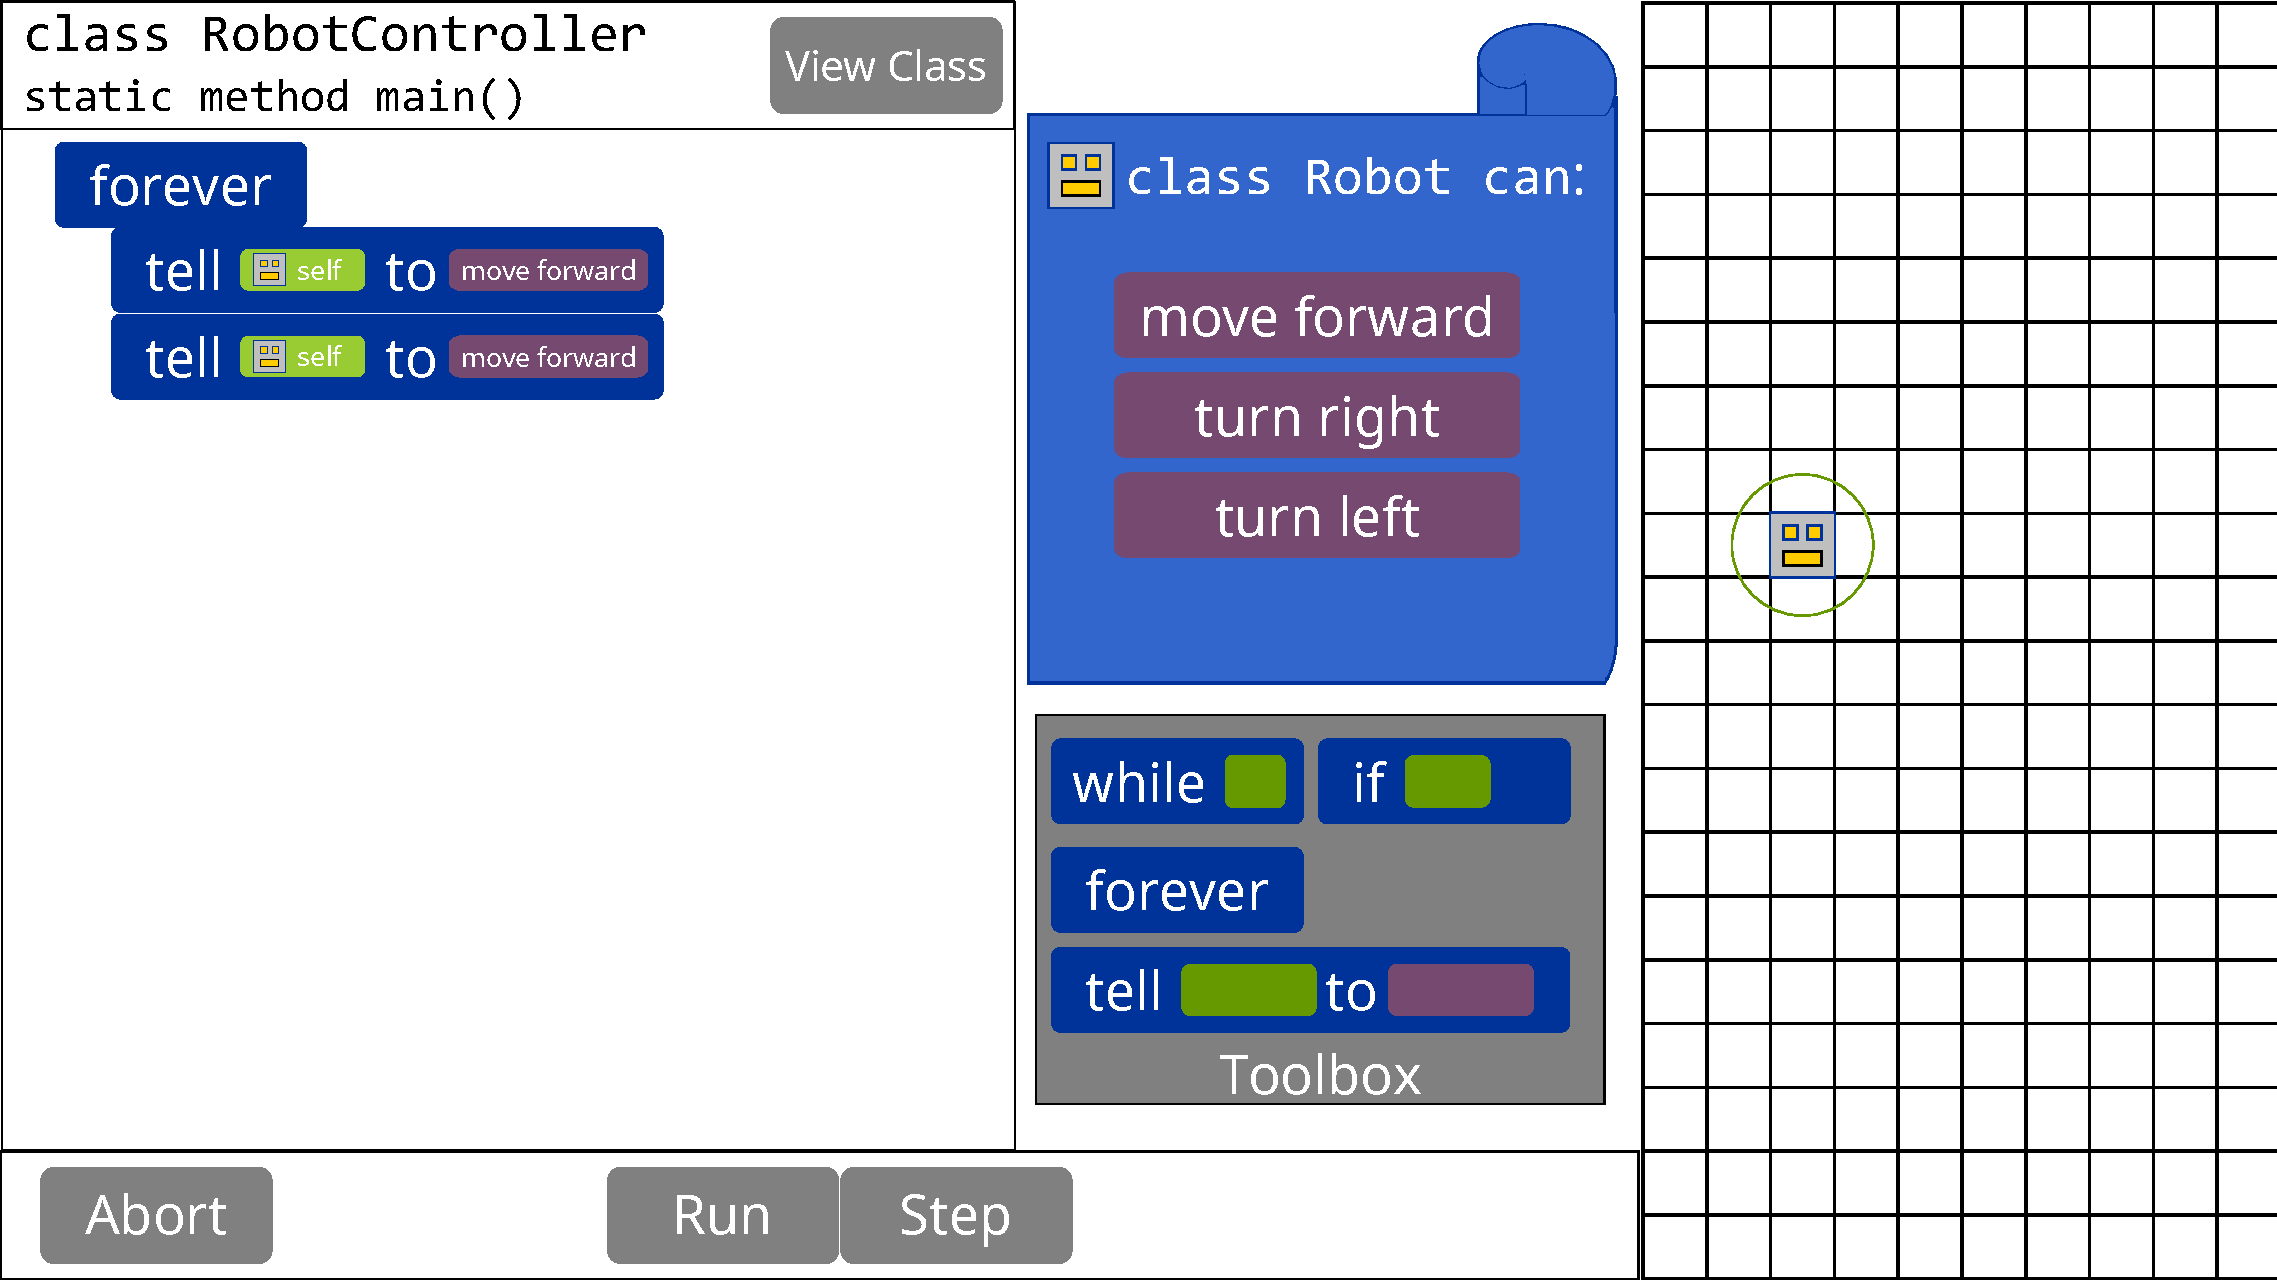
\includegraphics[width=\textwidth]{mockup.pdf}
  \caption{The main game interface.}
\end{figure}

The user interface has three main components: the world map, the
visual programmer and the interactive debugger. Normally, the student
will see only the programming and map interface. Once the student runs
their code, the debugger will appear, tracing the execution of the
code blocks in tandem with their effect on the world map. Based on
feedback from the paper prototype, we removed the interactive Java
debugger, as students would likely ignore it. Instead, we plan to fade
Java code into the blocks themselves while executing, mixing in more
actual code with the blocks as the game progresses.

Here the ``blueprint'' metaphor shows the student what methods are
available, and the object instance they are controlling is highlighted
on the map. The \texttt{self} block (\texttt{this} in Java) is
annotated with the same picture as the blueprint and map.

\subsection{Level Design and Progression}

Our rough concept progression can be found in figure~\ref{fig:progression}.

\begin{figure}[h]
  \centering
  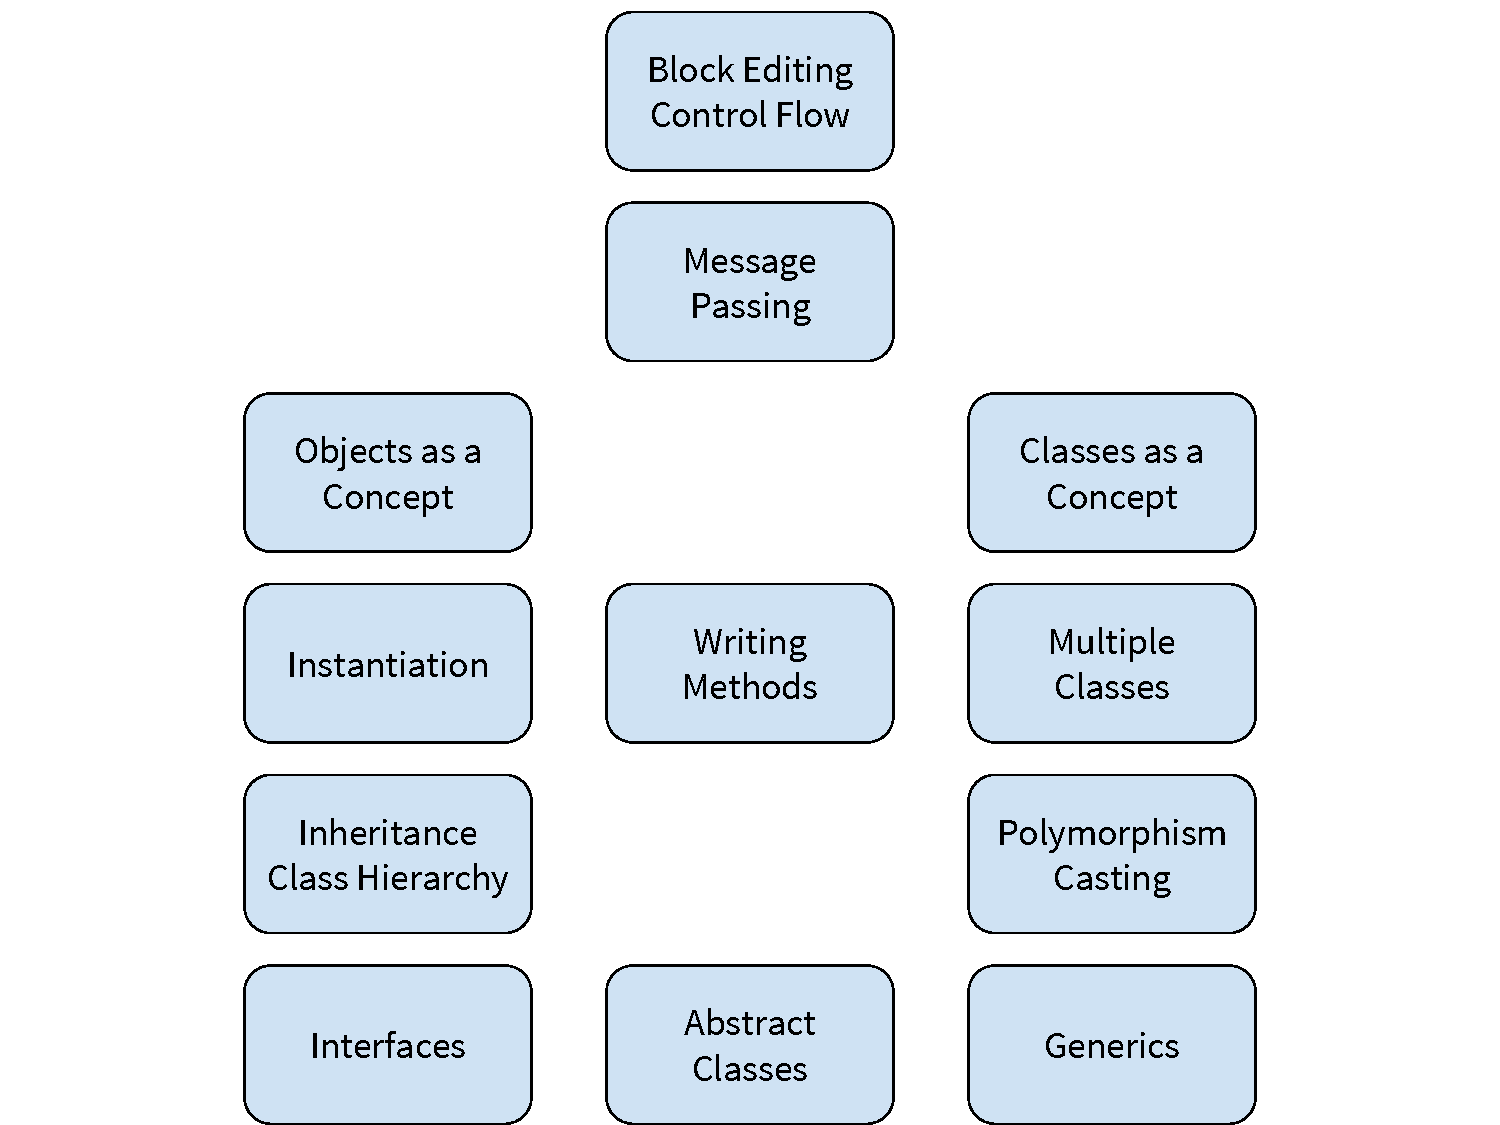
\includegraphics[width=\textwidth]{concept_progression.pdf}
  \caption{The concept progression. Items within a row do not
    necessarily depend on each other, but each row depends on the
    concepts in the previous row.}\label{fig:progression}
\end{figure}

The game will begin and feature a series of interactive
tutorials. When introducing a concept, students will be guided through
using the new idea TODO finish sentence. In particular, most block
types and capabilities will be slowly introduced, based on feedback
from the paper prototype, where the function and intent of many blocks
was unclear when presented without some sort of accompanying
explanation.

% What are the actions that the player can take in the game? What will
% be the result of these actions?

% What will the challenges look like?  What will the player
% specifically be asked to do?
As for the challenges themselves,

% How will your game decide whether object-oriented code the player
% has constructed is correct? Will correctness be based purely on
% whether the code performs the desired task, or will you also add
% constraints to enforce object-orientedness? How would this be done?
Our system simply requires the student to accomplish the given
objectives, using the tools given to them. Judging object-orientedness
TODO. However, the intent is to construct puzzles such that a
non-object-oriented solution is tedious or unappealing; for instance,
a robot may lack a \texttt{turnRight()} method, and students would be
encouraged to define one. While they do not necessarily have to,

% How will the game increase in difficulty? What will an easy, medium,
% and hard challenge look like?
In terms of difficulty,

\section{Prior Work}

Compared to prior systems like
Scratch\footnote{https://scratch.mit.edu/} and
Lightbot\footnote{http://lightbot.com/hour-of-code-2015-flash.html},
our system will explicitly model object-oriented concepts. For
instance, LightBot provides a fixed set of actions that implicitly
operate on the robot and space for a single subroutine. In contrast,
our system would allow user-defined methods on multiple classes, as
well as multiple different types of objects and control over multiple
objects simultaneously. Compared to Scratch, while our block system is
(intentionally) modeled after theirs, again, our system explicitly
shows the objects and methods being invoked, while in Scratch scripts
are attached to a particular sprite and implicitly act on that
sprite. In other words, while Scratch has all actions take place on
\texttt{this}, our system will show \texttt{this} as well as other
objects and allow the user to manipulate them at will.

\section{Evaluation}

We intend to test the system with a group of students in a class such
as CS 2110, Advanced Placement Computer Science, or similar class
involving Java and object-oriented principles. Students could be given
a pre- and post- test asking about various concepts from this
paradigm. As noted from feedback on the paper prototype, finding an
appropriate target audience is difficult---we need students who have
some programming basics, but who have not fully learned OOP.\@ TODO:
solution.

\section{Milestones}

\subsection{Alpha}

\begin{itemize}
\item
\end{itemize}

\begin{tabu}{lXXl}
\toprule
Task & Priority & Person & Hours \\
\midrule
Task description & Must/should/could have & Person & Hours \\
\bottomrule
\end{tabu}

\subsection{Beta}

\begin{itemize}
\item
\end{itemize}

\subsection{Final}
\begin{itemize}
\item
\end{itemize}

\end{document}
